\documentclass[]{beamer}
\usepackage{beamerthemesplit}
\usepackage{graphics}
\usepackage{pstricks}
\usepackage{graphicx}
\usepackage{hyperref}
\usepackage{subfigure}
\usepackage{listings}
\usepackage{courier}
\usepackage{multirow}
\usepackage{xspace}
\usepackage{tikz}


\mode<presentation>
{ \usetheme{Boadilla}
  \setbeamercovered{transparent}
  \setbeamertemplate{items}[square]
  \setbeamertemplate{theorems}[numbered]
  \setbeamertemplate{footline}[frame number]
}
 
%\useinnertheme[shadow=true]{rounded}
\useoutertheme{shadow}
\usecolortheme{whale}

\newcommand\blfootnote[1]{
  \begingroup
  \renewcommand\thefootnote{}\footnote{#1}
  \addtocounter{footnote}{-1}
  \endgroup
}

\mode
<all>

\title{C Programming}
\author{Wan-Lei Zhao}

\makeatletter
\DeclareRobustCommand\onedot{\futurelet\@let@token\@onedot}
\def\@onedot{\ifx\@let@token.\else.\null\fi\xspace}
\makeatother

\begin{document}
\begin{frame}
   \begin{center}
    \vspace{24pt}
    \Huge\textbf{C Programming}\blfootnote{Email: wlzhao@xmu.edu.cn, copyrights are fully reserved by the author.}\\
     \Huge{Lecture 2: Primitive} \\ \Huge{Data Types \& Expressions}
      \begin{figure}
     	\begin{center}
     		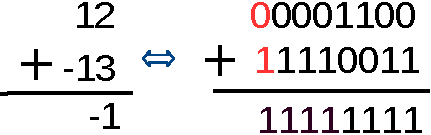
\includegraphics[width=0.3\linewidth]{figs/cover_lec2.pdf}
     	\end{center}
     \end{figure}
    \vspace{36pt}
  \end{center}
  \begin{align*}
   \vspace{18pt}
      \large{\mbox{Lecturer:}~Dr.~\mbox{Wan-Lei~~Zhao}} \\
      \large{Spring~~Semester~~2022} \\
   \vspace{30pt}
  \end{align*}
\end{frame}

\definecolor{cornblue}{HTML}{6495ED}
\definecolor{navyblue}{HTML}{000080}
\definecolor{midnblue}{HTML}{191970}
\definecolor{lghtblue}{HTML}{B0C4DE}
\setbeamercolor{background}{fg=black, bg=lghtblue}
\setbeamercolor{palette primary}{fg=white, bg=lghtblue}
\setbeamercolor{palette secondary}{fg=black, bg=cornblue}
\setbeamercolor{palette tertiary}{fg=black, bg=lghtblue}
\setbeamercolor{palette quaternary}{fg=black, bg=lghtblue}
\setbeamercolor{frametitle}{fg=black, bg=white}
\definecolor{ballblue}{rgb}{0.13, 0.67, 0.8}
\definecolor{cornflowerblue}{rgb}{0.39,0.58,0.93}
\definecolor{babyblueeyes}{rgb}{0.63, 0.79, 0.95}

\setbeamertemplate{footline}
{
  \leavevmode%
  \hbox{%
  \begin{beamercolorbox}[wd=.275\paperwidth,ht=2.25ex,dp=1ex,center]{author in head/foot}%
    \usebeamerfont{author in head/foot}\insertshortauthor
  \end{beamercolorbox}%
  \begin{beamercolorbox}[wd=.44\paperwidth,ht=2.25ex,dp=1ex,center]{title in head/foot}%
    \usebeamerfont{title in head/foot}\insertshorttitle\hspace*{3em}
    \hspace*{1ex}
  \end{beamercolorbox}%
  \begin{beamercolorbox}[wd=.285\paperwidth,ht=2.25ex,dp=1ex,center]{date/foot}%
    \usebeamerfont{title in head/foot}\hspace*{2em}
    \insertframenumber{} / \inserttotalframenumber\hspace*{1ex}
  \end{beamercolorbox}}%
  \vskip0pt
}



% preset-listing options
\lstset{
  backgroundcolor=\color{white},   
  basicstyle=\footnotesize,    
  language=c,
  breakatwhitespace=false,         
  breaklines=true,                 % sets automatic line breaking
  captionpos=b,                    % sets the caption-position to bottom
  commentstyle=\color{ballblue},    % comment style
  extendedchars=true,              
  frame=single,                    % adds a frame around the code     
  keywordstyle=\color{blue},       % keyword style
  numbers=left,                    
  numbersep=5pt,                   
  numberstyle=\tiny\color{blue}, 
  rulecolor=\color{babyblueeyes},
  stepnumber=1,              
  stringstyle=\color{black},     % string literal style
  tabsize=4,                       % sets default tabsize to 4 spaces
  title=\lstname                   
}


\section{Basics about Data Representation}
\label{sec:basic}
\begin{frame}<beamer>
    \frametitle{Outline}
    \tableofcontents[currentsection]
\end{frame}


\begin{frame}
\frametitle{Everything is binary code in computer (1)}
	\begin{itemize}
		\item {Everything in computer is in \textbf{binary} form}
		\item {Data: integers, real numbers and strings}
		\item {Instructions}
		\item {Addresses: sequential numbers for the memory cells}
	\end{itemize}
	\begin{itemize}
		\item {It is therefore necessary to know how the binary code is produced}
		\item {In addition, for convenience}
		\item {\textbf{Octal} and \textbf{Hexadecimal} numbers are also used for display}
	\end{itemize}
\end{frame}

\begin{frame}{Everything is binary code in computer (2)}
	\begin{figure}
			
\includegraphics[width=0.6\linewidth]{figs/matrix.pdf}
	\end{figure}
	\begin{itemize}
		\item {Anyone watched this movie?}
	\end{itemize}
\end{frame}

\begin{frame}
\frametitle{Decimal to Binary, Octal and Hexadecimal (1)}
	\begin{figure}
		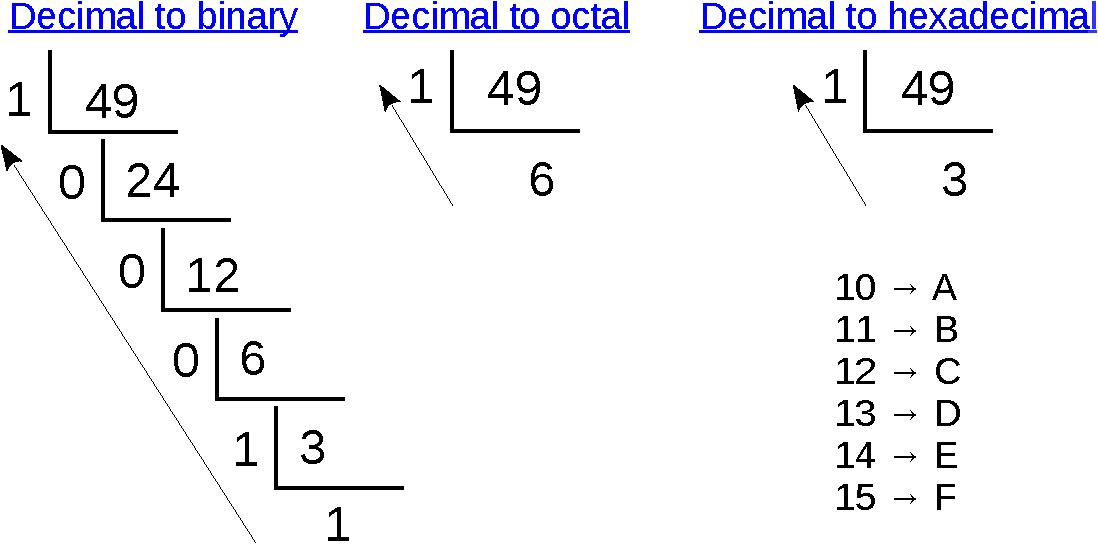
\includegraphics[width=0.75\linewidth]{figs/d2b.pdf}
	\end{figure}
	\begin{itemize}
		\item {Binary code: $110001_{(2)}$}
		\item {Octal code: $61_{(8)}$}
		\item {Hexadecimal code: $31_{(16)}$}
		\item {Can you figure out the relation between them}
	\end{itemize}
\end{frame}

\begin{frame}
\frametitle{Decimal to Binary, Octal and Hexadecimal (2)}
	\begin{itemize}
		\item {Try it by yourself to convert \textbf{60} to}
		\begin{itemize}
			\item {Binary code: }
			\item {Octal code: }
			\item {Hexadecimal code: }
		\end{itemize}
	\end{itemize}
\end{frame}

\begin{frame}
\frametitle{Decimal to Binary, Octal and Hexadecimal (2)}
	\begin{itemize}
		\item {Try it by yourself to convert \textbf{60} to}
		\item {Binary code: $111100_{(2)}$}
		\item {Octal code: $74_{(8)}$}
		\item {Hexadecimal code: $3C_{(16)}$}
	\end{itemize}
\end{frame}

\begin{frame}
\frametitle{Decimal to Binary, Octal and Hexadecimal (3)}
	\begin{figure}
		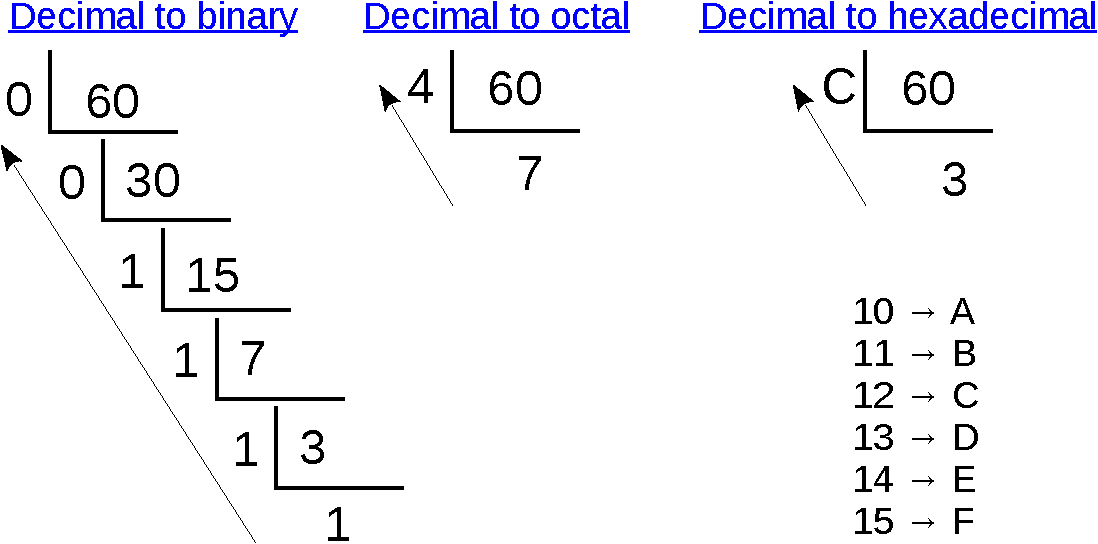
\includegraphics[width=0.75\linewidth]{figs/d2b_v2.pdf}
	\end{figure}
\end{frame}

\begin{frame}
\frametitle{Decimal to Binary, Octal and Hexadecimal (4)}
	\begin{figure}
		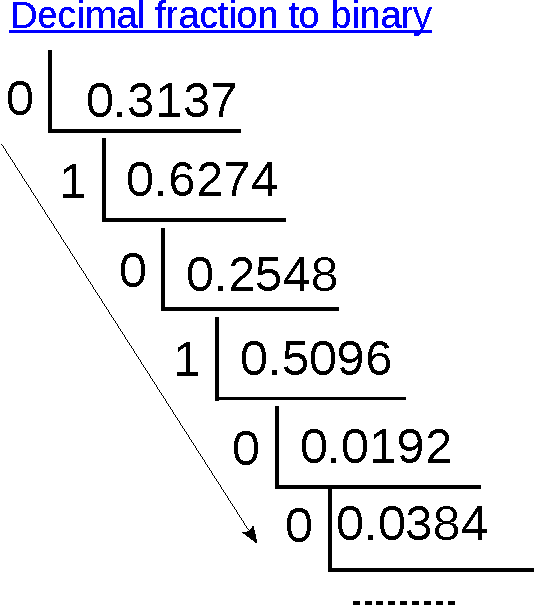
\includegraphics[width=0.45\linewidth]{figs/d2b1.pdf}
	\end{figure}
\begin{equation}
0{\times}2^{-1}+1{\times}2^{-2}+0{\times}2^{-3}+1{\times}2^{-4}=0.3125 \approx 0.3137 \nonumber
\end{equation}
\end{frame}

\begin{frame}
\frametitle{Binary, Octal and Hexadecimal to Decimal}
	\begin{itemize}
		\item {Binary code: $111100_{(2)}$}
		\item {Octal code: $74_{(8)}$}
		\item {Hexadecimal code: $3C_{(16)}$}
	\end{itemize}
	\begin{eqnarray}
		1\times2^5+1\times2^4+1\times2^3+1\times2^2+0\times2^1+0\times2^0=60 \nonumber \\
		7\times8^1+4\times8^0=60 \nonumber \\
		3\times16^1+12\times16^0=60 \nonumber
	\end{eqnarray}
\end{frame}


\begin{frame}
 \frametitle{Data in the memory (1)}
\begin{itemize}
	\item {Data in the memory is kept in binary form}
	\item {Given an integer \textbf{49}, its binary code is $110001_{(2)}$}
	\item {It is kept in following form}
\end{itemize}
\vspace{0.1in}
\begin{center}
\begin{tikzpicture}[font=\small,x=1.4cm]
		\begin{uncoverenv}<1->
			\node[red, below=.4em, right=0em, ] at (0,1.9) {0};
			\draw[blue] (0,1.6) -- (.5,1.6);
			\draw[blue] (.5,1.6) -- (.5,1.9);
			\draw[blue] (0,1.9) -- (.5,1.9);
			\draw[blue] (0,1.6) -- (0,1.9);
		
			\node[blue, below=.4em, right=0em, ] at (.5,1.9) {1};
			\draw[blue] (.5,1.6) -- (1,1.6);
			\draw[blue] (1,1.6) -- (1,1.9);
			\draw[blue] (.5,1.9) -- (1,1.9);
			\draw[blue] (.5,1.6) -- (.5,1.9);
			
			\node[blue, below=.4em, right=0em, ] at (1,1.9) {1};
			\draw[blue] (1,1.6) -- (1.5,1.6);
			\draw[blue] (1.5,1.6) -- (1.5,1.9);
			\draw[blue] (1,1.9) -- (1.5,1.9);
			\draw[blue] (1,1.6) -- (1,1.9);
		
			\node[blue, below=.4em, right=0em, ] at (1.5,1.9) {0};
			\draw[blue] (1.5,1.6) -- (2,1.6);
			\draw[blue] (2,1.6) -- (2,1.9);
			\draw[blue] (1.5,1.9) -- (2,1.9);
			\draw[blue] (1.5,1.6) -- (1.5,1.9);

			\node[blue, below=.4em, right=0em, ] at (2,1.9) {0};
			\draw[blue] (2,1.6) -- (2.5,1.6);
			\draw[blue] (2.5,1.6) -- (2.5,1.9);
			\draw[blue] (2,1.9) -- (2.5,1.9);
			\draw[blue] (2,1.6) -- (2,1.9);

			\node[blue, below=.4em, right=0em, ] at (2.5,1.9) {0};
			\draw[blue] (2.5,1.6) -- (3,1.6);
			\draw[blue] (3,1.6) -- (3,1.9);
			\draw[blue] (2.5,1.9) -- (3,1.9);
			\draw[blue] (2.5,1.6) -- (2.5,1.9);
			
			\node[blue, below=.4em, right=0em, ] at (3,1.9) {1};
			\draw[blue] (3,1.6) -- (3.5,1.6);
			\draw[blue] (3.5,1.6) -- (3.5,1.9);
			\draw[blue] (3,1.9) -- (3.5,1.9);
			\draw[blue] (3,1.6) -- (3,1.9);
		\end{uncoverenv}
	\end{tikzpicture}
\end{center}
\begin{itemize}
	\item {Given an integer \textbf{-49}, its binary code is \textcolor{red}{1}$110001_{(2)}$}
	\item {It is kept in following form}
\end{itemize}
\begin{center}
\begin{tikzpicture}[font=\small,x=1.4cm]
		\begin{uncoverenv}<1->
			\node[red, below=.4em, right=0em, ] at (0,1.9) {1};
			\draw[blue] (0,1.6) -- (.5,1.6);
			\draw[blue] (.5,1.6) -- (.5,1.9);
			\draw[blue] (0,1.9) -- (.5,1.9);
			\draw[blue] (0,1.6) -- (0,1.9);
		
			\node[blue, below=.4em, right=0em, ] at (.5,1.9) {1};
			\draw[blue] (.5,1.6) -- (1,1.6);
			\draw[blue] (1,1.6) -- (1,1.9);
			\draw[blue] (.5,1.9) -- (1,1.9);
			\draw[blue] (.5,1.6) -- (.5,1.9);
			
			\node[blue, below=.4em, right=0em, ] at (1,1.9) {1};
			\draw[blue] (1,1.6) -- (1.5,1.6);
			\draw[blue] (1.5,1.6) -- (1.5,1.9);
			\draw[blue] (1,1.9) -- (1.5,1.9);
			\draw[blue] (1,1.6) -- (1,1.9);
		
			\node[blue, below=.4em, right=0em, ] at (1.5,1.9) {0};
			\draw[blue] (1.5,1.6) -- (2,1.6);
			\draw[blue] (2,1.6) -- (2,1.9);
			\draw[blue] (1.5,1.9) -- (2,1.9);
			\draw[blue] (1.5,1.6) -- (1.5,1.9);

			\node[blue, below=.4em, right=0em, ] at (2,1.9) {0};
			\draw[blue] (2,1.6) -- (2.5,1.6);
			\draw[blue] (2.5,1.6) -- (2.5,1.9);
			\draw[blue] (2,1.9) -- (2.5,1.9);
			\draw[blue] (2,1.6) -- (2,1.9);

			\node[blue, below=.4em, right=0em, ] at (2.5,1.9) {0};
			\draw[blue] (2.5,1.6) -- (3,1.6);
			\draw[blue] (3,1.6) -- (3,1.9);
			\draw[blue] (2.5,1.9) -- (3,1.9);
			\draw[blue] (2.5,1.6) -- (2.5,1.9);
			
			\node[blue, below=.4em, right=0em, ] at (3,1.9) {1};
			\draw[blue] (3,1.6) -- (3.5,1.6);
			\draw[blue] (3.5,1.6) -- (3.5,1.9);
			\draw[blue] (3,1.9) -- (3.5,1.9);
			\draw[blue] (3,1.6) -- (3,1.9);
		\end{uncoverenv}
	\end{tikzpicture}
\end{center}
\begin{itemize}
	\item {The highest bit is reserved for sign}
	\item {This is true for \textbf{real} numbers later we will see}
	\item {We use 8 bits (1 byte), 2 bytes or more bytes to keep a number}
\end{itemize}

\begin{center}
\begin{tikzpicture}[font=\small,x=1.4cm]
		\begin{uncoverenv}<1->
			\node[red, below=.4em, right=0em, ] at (0,1.9) {1};
			\draw[blue] (0,1.6) -- (.5,1.6);
			\draw[blue] (.5,1.6) -- (.5,1.9);
			\draw[blue] (0,1.9) -- (.5,1.9);
			\draw[blue] (0,1.6) -- (0,1.9);

			\node[blue, below=.4em, right=0em, ] at (0.5,1.9) {0};
			\draw[blue] (.5,1.6) -- (1,1.6);
			\draw[blue] (1,1.6) -- (1,1.9);
			\draw[blue] (.5,1.9) -- (1,1.9);
			\draw[blue] (.5,1.6) -- (.5,1.9);
		
			\node[blue, below=.4em, right=0em, ] at (1.0,1.9) {1};
			\draw[blue] (1,1.6) -- (1.5,1.6);
			\draw[blue] (1.5,1.6) -- (1.5,1.9);
			\draw[blue] (1,1.9) -- (1.5,1.9);
			\draw[blue] (1,1.6) -- (1,1.9);
			
			\node[blue, below=.4em, right=0em, ] at (1.5,1.9) {1};
			\draw[blue] (1.5,1.6) -- (2,1.6);
			\draw[blue] (2,1.6) -- (2,1.9);
			\draw[blue] (1.5,1.9) -- (2,1.9);
			\draw[blue] (1.5,1.6) -- (1.5,1.9);
		
			\node[blue, below=.4em, right=0em, ] at (2.0,1.9) {0};
			\draw[blue] (2,1.6) -- (2.5,1.6);
			\draw[blue] (2.5,1.6) -- (2.5,1.9);
			\draw[blue] (2,1.9) -- (2.5,1.9);
			\draw[blue] (2,1.6) -- (2,1.9);

			\node[blue, below=.4em, right=0em, ] at (2.5,1.9) {0};
			\draw[blue] (2.5,1.6) -- (3,1.6);
			\draw[blue] (3,1.6) -- (3,1.9);
			\draw[blue] (2.5,1.9) -- (3,1.9);
			\draw[blue] (2.5,1.6) -- (2.5,1.9);

			\node[blue, below=.4em, right=0em, ] at (3.0,1.9) {0};
			\draw[blue] (3,1.6) -- (3.5,1.6);
			\draw[blue] (3.5,1.6) -- (3.5,1.9);
			\draw[blue] (3,1.9) -- (3.5,1.9);
			\draw[blue] (3,1.6) -- (3,1.9);
			
			\node[blue, below=.4em, right=0em, ] at (3.5,1.9) {1};
			\draw[blue] (3.5,1.6) -- (4,1.6);
			\draw[blue] (4,1.6) -- (4,1.9);
			\draw[blue] (3.5,1.9) -- (4,1.9);
			\draw[blue] (3.5,1.6) -- (3.5,1.9);
		\end{uncoverenv}
	\end{tikzpicture}
\end{center}

\end{frame}

\begin{frame}
 \frametitle{Data in the memory (2)}
\begin{itemize}
	\item {Data in the memory is kept in binary form}
	\item {Given we have several numbers to be kept}
	\item {They are kept one after another (assume we use 1 byte for one number)}
\end{itemize}
\begin{center}
\begin{tikzpicture}[font=\small,x=1.4cm]
		\begin{uncoverenv}<1->
			\node[black, below=.4em, right=0em, ] at (-0.8,1.9) {0000};
			\node[red, below=.4em, right=0em, ] at (0,1.9) {1};
			\draw[blue] (0,1.6) -- (.5,1.6);
			\draw[blue] (.5,1.6) -- (.5,1.9);
			\draw[blue] (0,1.9) -- (.5,1.9);
			\draw[blue] (0,1.6) -- (0,1.9);

			\node[black, below=.4em, right=0em, ] at (-0.8,1.5) {0001};
			\node[red, below=.4em, right=0em, ] at (0,1.5) {0};
			\draw[blue] (0,1.2) -- (.5,1.2);
			\draw[blue] (.5,1.2) -- (.5,1.5);
			\draw[blue] (0,1.5) -- (.5,1.5);
			\draw[blue] (0,1.2) -- (0,1.5);

			\node[black, below=.4em, right=0em, ] at (-0.8,1.1) {0002};
			\node[black, below=.4em, right=0em, ] at (-0.8,0.7) {0003};
			\node[red, below=.4em, right=0em, ] at (0,1.1) {0};
			\draw[blue] (0,0.8) -- (.5,0.8);
			\draw[blue] (.5,0.8) -- (.5,1.1);
			\draw[blue] (0,1.1) -- (.5,1.1);
			\draw[blue] (0,0.8) -- (0,1.1);
			%%1st bit

			\node[blue, below=.4em, right=0em, ] at (0.5,0.7) {.};
			\node[blue, below=.4em, right=0em, ] at (0.5,1.9) {0};
			\draw[blue] (.5,1.6) -- (1,1.6);
			\draw[blue] (1,1.6) -- (1,1.9);
			\draw[blue] (.5,1.9) -- (1,1.9);
			\draw[blue] (.5,1.6) -- (.5,1.9);

			\node[blue, below=.4em, right=0em, ] at (0.5,1.5) {0};
			\draw[blue] (.5,1.2) -- (1,1.2);
			\draw[blue] (1,1.2) -- (1,1.5);
			\draw[blue] (.5,1.5) -- (1,1.5);
			\draw[blue] (.5,1.2) -- (.5,1.5);

			\node[blue, below=.4em, right=0em, ] at (0.5,1.1) {1};
			\draw[blue] (.5,0.8) -- (1,0.8);
			\draw[blue] (1,0.8) -- (1,1.1);
			\draw[blue] (.5,1.1) -- (1,1.1);
			\draw[blue] (.5,0.8) -- (.5,1.1);
			%%2nd bit

			\node[blue, below=.4em, right=0em, ] at (1.0,0.7) {.};		
			\node[blue, below=.4em, right=0em, ] at (1.0,1.9) {1};
			\draw[blue] (1,1.6) -- (1.5,1.6);
			\draw[blue] (1.5,1.6) -- (1.5,1.9);
			\draw[blue] (1,1.9) -- (1.5,1.9);
			\draw[blue] (1,1.6) -- (1,1.9);

			\node[blue, below=.4em, right=0em, ] at (1.0,1.5) {1};
			\draw[blue] (1,1.2) -- (1.5,1.2);
			\draw[blue] (1.5,1.2) -- (1.5,1.5);
			\draw[blue] (1,1.5) -- (1.5,1.5);
			\draw[blue] (1,1.2) -- (1,1.5);
		
			\node[blue, below=.4em, right=0em, ] at (1.0,1.1) {0};
			\draw[blue] (1,0.8) -- (1.5,0.8);
			\draw[blue] (1.5,0.8) -- (1.5,1.1);
			\draw[blue] (1,1.1) -- (1.5,1.1);
			\draw[blue] (1,0.8) -- (1,1.1);
			%%3rd
			
			\node[blue, below=.4em, right=0em, ] at (1.5,1.9) {1};
			\draw[blue] (1.5,1.6) -- (2,1.6);
			\draw[blue] (2,1.6) -- (2,1.9);
			\draw[blue] (1.5,1.9) -- (2,1.9);
			\draw[blue] (1.5,1.6) -- (1.5,1.9);

			\node[blue, below=.4em, right=0em, ] at (1.5,1.5) {1};
			\draw[blue] (1.5,1.2) -- (2,1.2);
			\draw[blue] (2,1.2) -- (2,1.5);
			\draw[blue] (1.5,1.5) -- (2,1.5);
			\draw[blue] (1.5,1.2) -- (1.5,1.5);
		
			\node[blue, below=.4em, right=0em, ] at (1.5,1.1) {1};
			\draw[blue] (1.5,0.8) -- (2,0.8);
			\draw[blue] (2,0.8) -- (2,1.1);
			\draw[blue] (1.5,1.1) -- (2,1.1);
			\draw[blue] (1.5,0.8) -- (1.5,1.1);
			%%4th
		
			\node[blue, below=.4em, right=0em, ] at (2.0,1.9) {0};
			\draw[blue] (2,1.6) -- (2.5,1.6);
			\draw[blue] (2.5,1.6) -- (2.5,1.9);
			\draw[blue] (2,1.9) -- (2.5,1.9);
			\draw[blue] (2,1.6) -- (2,1.9);

			\node[blue, below=.4em, right=0em, ] at (2.0,1.5) {0};
			\draw[blue] (2,1.2) -- (2.5,1.2);
			\draw[blue] (2.5,1.2) -- (2.5,1.5);
			\draw[blue] (2,1.5) -- (2.5,1.5);
			\draw[blue] (2,1.2) -- (2,1.5);
			
			\node[blue, below=.4em, right=0em, ] at (2.0,1.1) {1};
			\draw[blue] (2,0.8) -- (2.5,0.8);
			\draw[blue] (2.5,0.8) -- (2.5,1.1);
			\draw[blue] (2,1.1) -- (2.5,1.1);
			\draw[blue] (2,0.8) -- (2,1.1);
			%%5th

			\node[blue, below=.4em, right=0em, ] at (2.5,1.9) {0};
			\draw[blue] (2.5,1.6) -- (3,1.6);
			\draw[blue] (3,1.6) -- (3,1.9);
			\draw[blue] (2.5,1.9) -- (3,1.9);
			\draw[blue] (2.5,1.6) -- (2.5,1.9);
			
			\node[blue, below=.4em, right=0em, ] at (2.5,1.5) {0};
			\draw[blue] (2.5,1.2) -- (3,1.2);
			\draw[blue] (3,1.2) -- (3,1.5);
			\draw[blue] (2.5,1.5) -- (3,1.5);
			\draw[blue] (2.5,1.2) -- (2.5,1.5);
			
			\node[blue, below=.4em, right=0em, ] at (2.5,1.1) {1};
			\draw[blue] (2.5,0.8) -- (3,0.8);
			\draw[blue] (3,0.8) -- (3,1.1);
			\draw[blue] (2.5,1.1) -- (3,1.1);
			\draw[blue] (2.5,0.8) -- (2.5,1.1);
			%%6th

			\node[blue, below=.4em, right=0em, ] at (3.0,1.9) {0};
			\draw[blue] (3,1.6) -- (3.5,1.6);
			\draw[blue] (3.5,1.6) -- (3.5,1.9);
			\draw[blue] (3,1.9) -- (3.5,1.9);
			\draw[blue] (3,1.6) -- (3,1.9);

			\node[blue, below=.4em, right=0em, ] at (3.0,1.5) {1};
			\draw[blue] (3,1.2) -- (3.5,1.2);
			\draw[blue] (3.5,1.2) -- (3.5,1.5);
			\draw[blue] (3,1.5) -- (3.5,1.5);
			\draw[blue] (3,1.2) -- (3,1.5);

			\node[blue, below=.4em, right=0em, ] at (3.0,1.1) {0};
			\draw[blue] (3,0.8) -- (3.5,0.8);
			\draw[blue] (3.5,0.8) -- (3.5,1.1);
			\draw[blue] (3,1.1) -- (3.5,1.1);
			\draw[blue] (3,0.8) -- (3,1.1);
			%%7th
			
			\node[blue, below=.4em, right=0em, ] at (3.5,1.9) {1};
			\draw[blue] (3.5,1.6) -- (4,1.6);
			\draw[blue] (4,1.6) -- (4,1.9);
			\draw[blue] (3.5,1.9) -- (4,1.9);
			\draw[blue] (3.5,1.6) -- (3.5,1.9);

			\node[blue, below=.4em, right=0em, ] at (3.5,1.5) {1};
			\draw[blue] (3.5,1.2) -- (4,1.2);
			\draw[blue] (4,1.2) -- (4,1.5);
			\draw[blue] (3.5,1.5) -- (4,1.5);
			\draw[blue] (3.5,1.2) -- (3.5,1.5);
			
			\node[blue, below=.4em, right=0em, ] at (3.5,1.1) {1};
			\draw[blue] (3.5,0.8) -- (4,0.8);
			\draw[blue] (4,0.8) -- (4,1.1);
			\draw[blue] (3.5,1.1) -- (4,1.1);
			\draw[blue] (3.5,0.8) -- (3.5,1.1);
		\end{uncoverenv}
	\end{tikzpicture}
\end{center}

\end{frame}

\begin{frame}
	\frametitle{Data in the memory (3)}
	\begin{itemize}
		\item {Now, think about an important issue}
		\item {Given 1 byte, how many different numbers we can represent}
		\item {Assuming no sign bit}
	\end{itemize}
	\begin{figure}
		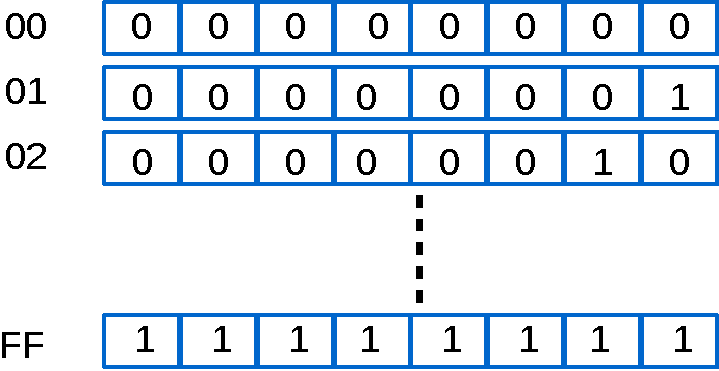
\includegraphics[width=0.55\linewidth]{figs/byte.pdf}
	\end{figure}
	\begin{itemize}
		\item {With 1 byte, there are \textbf{$2^8=256$} numbers}
		\item {Since our memory are limited, we can only represent a limited range of numbers}
	\end{itemize}
\end{frame}


\begin{frame}
	\frametitle{Data in the memory (4)}
	\begin{itemize}
		\item {Now, think about how many different numbers we have if one bit is reserved for sign}
		\item {????}
	\end{itemize}
\end{frame}

\begin{frame}
	\frametitle{Data in the memory (5)}
	\begin{itemize}
		\item {Now, think about how many different numbers we have if one bit is reserved for sign}
		\item {$2{\times}2^7-1=255$}
		\item {Only 127 positive numbers (1 $\sim$ 127)}
		\item {127 negatives (-1 $\sim$ -127)}
	\end{itemize}
	\begin{itemize}
		\item {Some numbers can only be approximately represented by binary code}
		\item {For example, \textbf{3.3137}}
		\item {$11.0101_{(2)}$}
	\end{itemize}
\end{frame}

\begin{frame}
	\frametitle{One's complement and Two's Complement}
\begin{table}
\begin{center}
\begin{tabular}{|c|c|c|c|}
\hline
Original & bits & One's Complement & Two's Complement \\ \hline
23   & \textcolor{red}{0}0010111 & \textcolor{red}{0}0010111 & \textcolor{red}{0}0010111 \\ \hline 
-23   & \textcolor{red}{1}0010111 & \textcolor{red}{1}1101000 & \textcolor{red}{1}1101001 \\ \hline \hline
33   & \textcolor{red}{0}0100001 & \textcolor{red}{0}0100001 & \textcolor{red}{0}0100001 \\ \hline
-33   & \textcolor{red}{1}0100001 & \textcolor{red}{1}1011110 & \textcolor{red}{1}1011111 \\ \hline  
\end{tabular}
\end{center}
\end{table}
\begin{itemize}
	\item {One's complement and two's complement of positive numbers are the same as original code}
	\item {For negative number, we do not inverse its sign bit}
	\item {Why we do so??}
	\begin{itemize}
		\item {It is very convenient when we do substraction}
		\item {Substraction is converted to add operation}
	\end{itemize}
	\item {Now please work out one's complement and two's complement of \textbf{-17}}
\end{itemize}
\end{frame}
\section{Data types}
\label{sec:dtype}
\begin{frame}<beamer>
    \frametitle{Outline}
    \tableofcontents[currentsection]
\end{frame}


\begin{frame}{Data Types Supported in C}
\begin{figure}
	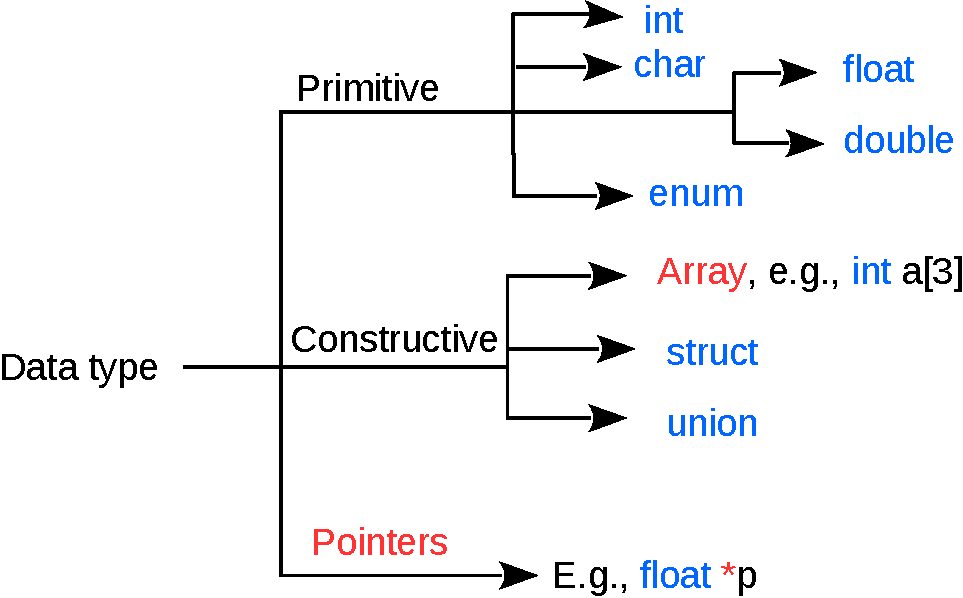
\includegraphics[width=0.75\linewidth]{figs/dtypes.pdf}
\end{figure}
\end{frame}

\begin{frame}[fragile]{Integer numbers}
	\begin{itemize}
		\item Keywords: \textcolor{blue}{int}, \textcolor{blue}{short}, \textcolor{blue}{long}
		\item Can be \textit{signed} (\textcolor{red}{default}) or \textit{unsigned}
		\item Actual size of \textit{int}, \textit{short}, \textit{long} depends on architecture
	\end{itemize}
	\begin{center}
	\begin{lstlisting}[language=c,frame=none, linewidth=0.85\linewidth]
 int a;	/*Range: -2,147,483,648 to 2,147,483,647*/
 short b;	/*Range: -32,768 to 32,767*/
 long c; /*Range: -2,147,483,648 to 2,147,483,647*/
 unsigned int a1;	/*Range: 0 to 4,294,967,297*/		
 unsigned short b1;	/*Range: 0 to 65,535*/
	\end{lstlisting}
	\end{center}	
	\begin{itemize}
		\item {\textcolor{blue}{int} and \textcolor{blue}{long} take 4 bytes (32 bits system)}
		\item {\textcolor{blue}{short} takes 2 bytes}
	\end{itemize}
\end{frame}

\begin{frame}[fragile]{Integer numbers}
	\vspace{-0.2in}
	\begin{itemize}
		\item Keywords: \textcolor{blue}{int}, \textcolor{blue}{short}, \textcolor{blue}{long}
		\item Can be \textit{signed} (\textcolor{red}{default}) or \textit{unsigned}
		\item Actual size of \textit{int}, \textit{short}, \textit{long} depends on architecture
	\end{itemize}
	%\vspace{-0.1in}
	\begin{figure}
		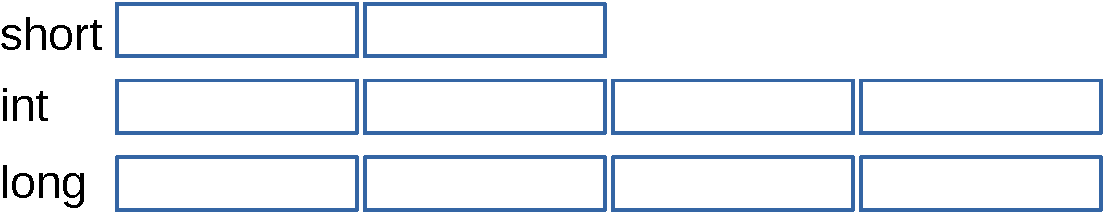
\includegraphics[width=0.65\linewidth]{figs/ints.pdf}
	\end{figure}
	\vspace{-0.1in}
	\begin{center}
	\begin{lstlisting}[language=c,frame=none, linewidth=0.9\linewidth]
 int a;	/*Range: -2,147,483,648 to 2,147,483,647*/
 short b;	/*Range: -32,768 to 32,767*/
 long c; /*Range: -2,147,483,648 to 2,147,483,647*/
 unsigned int a1;	/*Range: 0 to 4,294,967,297*/		
 unsigned short b1;	/*Range: 0 to 65,535*/
	\end{lstlisting}
	\end{center}	
\end{frame}


\begin{frame}[fragile]{Integer numbers}
	\begin{center}
		\begin{lstlisting}[numbers=none, frame=none, language=c]
	    int main()
	    {
	       short a = 0x8000;
	       short b = 0x7FFF;
	       short c = 0xFFFE;
	       char  d = 0x80;
	       printf("a = %d, b = %d, c = %d\n", a, b, c);
	       printf("d = %d\n", d);
	       return 0;
	    }
	\end{lstlisting}
	\end{center}	
\end{frame}

\begin{frame}[fragile]
	\frametitle{The Problem of Overflow (1)}
\begin{itemize}
	\item {Given following code, anything wrong??}
\end{itemize}
		\begin{lstlisting}[numbers=none, frame=none, language=c]
	    int main()
	    {
	       unsigned short b = 65537;
	       return 0;
	    }
	\end{lstlisting}
\end{frame}

\begin{frame}[fragile]
	\frametitle{The Problem of Overflow (2)}
\begin{itemize}
	\item {Given following code, anything wrong??}
\end{itemize}
		\begin{lstlisting}[numbers=none, language=c,frame=none]
	    int main()
	    {
	       unsigned short b = 65537;
	       return 0;
	    }
	\end{lstlisting}
	\vspace{-0.15in}
	\begin{itemize}
		\item {\textbf{b} will never reach to \textbf{65537}}
		\item {In this case, it is \textbf{65535}}
		\item {Guess the value of b in following code}
	\end{itemize}
		\begin{lstlisting}[numbers=none, language=c,frame=none]
	    int main()
	    {
	       short b = 65537;
	       return 0;
	    }
	\end{lstlisting}
\end{frame}

\begin{frame}[fragile]
	\frametitle{The Problem of Overflow (3)}
	\begin{itemize}
		\item {The same problem exists for \textcolor{red}{all primitive data types}}
		\item {Because, we only use limited bytes to represent the data}
		\item {Be careful when you assign big value to a variable}
		\item {Tricks: \underline{estimate how big it could be}}
	\end{itemize}

\end{frame}

\begin{frame}[fragile]{Floating point numbers (1)}
	\begin{itemize}
		\item {Keywords: \textcolor{blue}{float}, \textcolor{blue}{double}, \textcolor{blue}{long double}}
		\item {Real numbers: $x \in R$}
		\begin{itemize}
			\item {Due to limited memory, only 4 bytes/8 bytes are used for float/double}
			\item {So it will not cover the whole range of $R$}
		\end{itemize}
	\end{itemize}
	\vspace{0.05in}
	\begin{figure}
		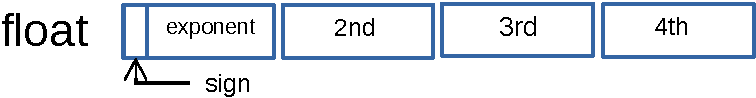
\includegraphics[width=0.5\linewidth]{figs/float.pdf}
	\end{figure}
	[\textbf{3.14159}]
	\begin{lstlisting}[language=c, numbers=none, basicstyle=\small, rulecolor=\color{black}]
	    0 0000100 110010010000111111001110
    ^     ^               ^
    |     |               |
    |     |               +--- significand = 0.7853975
    |     |
    |     +------------------- exponent = 4
    |
    +------------------------- sign = 0 (positive)
	\end{lstlisting}
	
\end{frame}

\begin{frame}[fragile]{Floating point numbers (2)}
	\begin{itemize}
		\item Keywords: \textcolor{blue}{float}, \textcolor{blue}{double}, \textcolor{blue}{long double}
	\end{itemize}
	\begin{lstlisting}[numbers=none, frame=none, language=c]
		float x = 0.125;			/*Precision: 7 to 8 digits*/
		double y = 111111.111111;	/*Precision: 15 to 16 digits*/
	\end{lstlisting}
	\vspace{-0.05in}
	\begin{itemize}
		\item {Now you should know a very useful operator \textcolor{blue}{sizeof}(.)}
	\end{itemize}
	\begin{lstlisting}[numbers=none, frame=none, language=c]
#include <stdio.h>
int main()
{
	float x = 0.125;
	double y = 111111.111111;
	printf("float: %d, double: %d", sizeof(x), sizeof(y));
}
	\end{lstlisting}
\end{frame}

\begin{frame}[fragile]{Characters (1)}
	\begin{itemize}
		\item Keyword: \textcolor{blue}{char}
		\item Can be \textcolor{red}{signed} (default) or \textcolor{blue}{unsigned}	
		\item Size: 1 Byte (8 bits) on almost every architecture
		\item Intended to represent a single character
		\item Stores its \textit{ASCII} number (e.g. 'A' $\Rightarrow$ 65)
	\end{itemize}
	\begin{itemize}
		\item {	You can define a \textcolor{blue}{char} either by its ASCII number or by its symbol:}	
	\end{itemize}
	\begin{lstlisting}[numbers=none, language=c]
		char a = 65;
		char b = 'A';	/*use single quotation marks*/
\end{lstlisting}
\end{frame}

\begin{frame}[fragile]{Characters (2)}
	\begin{itemize}
		\item {Essentially, \textcolor{blue}{char} uses 1 byte to represent 255 characters}
		\item {Each integer is associated with a character}
		\item {American Standard Code for Information Interchange (ASCII)}
	\end{itemize}
	\vspace{-0.06in}
	\begin{figure}
		\centering
		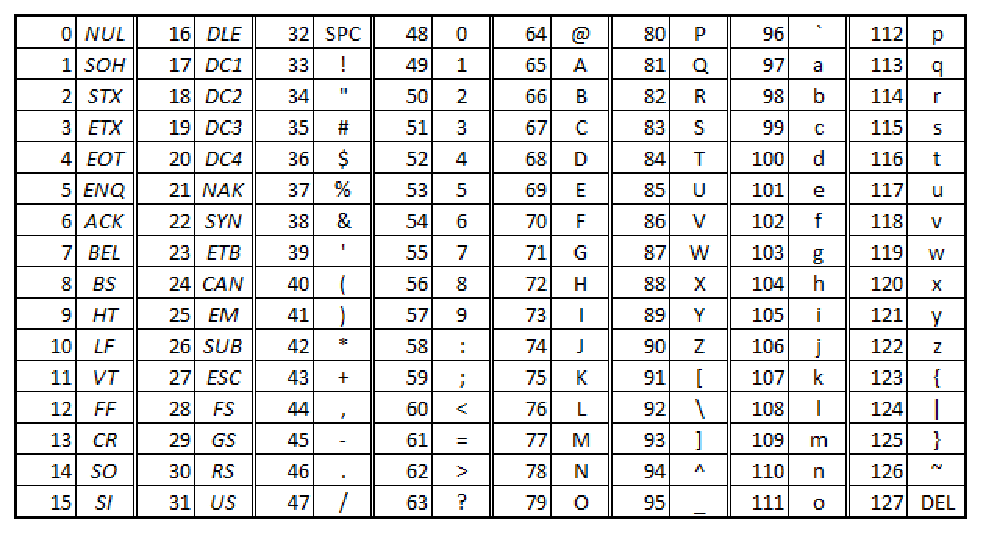
\includegraphics[width=0.8\linewidth]{figs/ascii.pdf}
	\end{figure}
\end{frame}

\begin{frame}[fragile]{Characters (3)}
	\begin{itemize}
		\item {There are some frequently used ones you should know}
	\end{itemize}
\begin{table}
\begin{tabular}{|c|c||c|c|}
\hline
ASCII & value & ASCII & value  \\ \hline
0$\sim$9 & 48$\sim$57 & A$\sim$Z & 65$\sim$90 \\ \hline
 a$\sim$z & 97$\sim$122 & $\llcorner\_\lrcorner$ & 32 \\ \hline
$\setminus$n & 10 & $\setminus$t & 9 \\ \hline
\end{tabular}
\end{table}
\begin{columns}
\begin{column}{0.60\linewidth}
	[\textbf{Code}]
	\begin{lstlisting}[language=c, numbers=none]
#include <stdio.h>
int main()
{
   printf("A: %d %c\n", 'A', 'A');
   printf("1: %d %c\n", '1', '1');
   printf("B: %d %c\n", 66, 66);
   printf("2: %d %c\n", 50, 50);
}
	\end{lstlisting}
\end{column}
\begin{column}{0.35\linewidth}
	[\textbf{Output}]
	\begin{lstlisting}[language=c, numbers=none]
	
	
	
	A: 65 A
	1: 49 1
	B: 66 B
	2: 50 2
	
	
	\end{lstlisting}
\end{column}
\end{columns}
\end{frame}

\begin{frame}[fragile]{Data type and its size}
\begin{figure}
	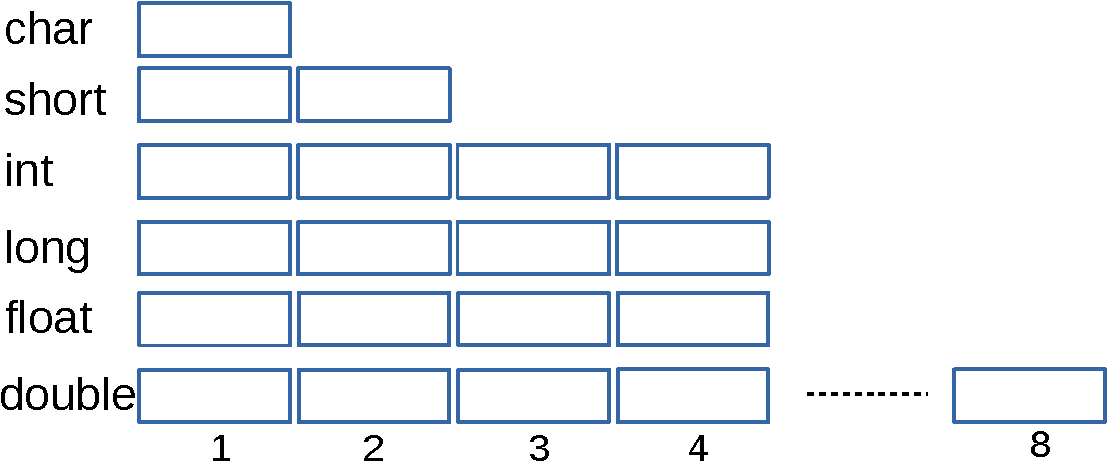
\includegraphics[width=0.85\linewidth]{figs/types.pdf}
\end{figure}
\begin{itemize}
	\item {You should clearly know what is the use of your data}
	\item {One should not define data in double/long double just for convenience}
	\item {It wastes a lot of memory}
	\item {String: an \textbf{array} of chars}
\end{itemize}
\end{frame}
\section{Visibility and Life-cycle of Variables}
\label{sec:vars}
\begin{frame}<beamer>
    \frametitle{Outline}
    \tableofcontents[currentsection]
\end{frame}

\begin{frame}[fragile]{Visibility and Life-cycle of Variables (1)}
\begin{itemize}
	\item {We take something for granted before}
	\item {Now we study them in detail}
	\begin{enumerate}
		\item {Could we use the same variable name in different functions?}
		\item {Could we use the same variable name in the same functions?}
		\item {Could different functions share the same variable?}
		\item {When a variable is born, when it dies??}
	\end{enumerate}
\end{itemize}

\end{frame}

\begin{frame}[fragile]{Visibility and Life-cycle of Variables (2)}
\begin{enumerate}
	\item {Could we use the same variable name in different functions?}
\end{enumerate}
\begin{columns}
\begin{column}{0.53\linewidth}
\begin{lstlisting}[linewidth=0.9\linewidth, xleftmargin=0.05\linewidth]
int func1(int n)
{
   int r = 3, a = 1;
   return (r*n+a);
}
float func2(int n, float a)
{
   float r = 1;
   int i = 0;
   for(i = 0; i < n; i++)
   {
      r = r*a;
   }
   return r;
}
\end{lstlisting}
\end{column}
\begin{column}{0.46\linewidth}
\begin{itemize}
	\item {The answer is \textcolor{red}{Yes}}
	\item {The visibility is inside function only}
	\item {It is born when the function is called}
	\item {It dies when calling is done}
\end{itemize}
\end{column}
\end{columns}
\end{frame}

\begin{frame}[fragile]{Visibility and Life-cycle of Variables (3)}
\begin{enumerate}
	\setcounter{enumi}{1}
	\item {Could we use the same variable name in the same function?}
\end{enumerate}
\begin{columns}
\begin{column}{0.55\linewidth}
\begin{lstlisting}[linewidth=0.9\linewidth, xleftmargin=0.05\linewidth]
float func2(int n, float a)
{
  float r = 1;
  int r = 0;
  int i = 0;
  float i = 0;
  for(i = 0; i < n; i++, r++)
  {
     r = r*a;
  }
  return r;
}
\end{lstlisting}
\end{column}
\begin{column}{0.44\linewidth}
\begin{itemize}
	\item {The answer is \textcolor{red}{No}}
	\item {Codes on the left cannot pass the compilation}
	\item {Basically, it is ambiguous}
	\item {Imagine there are two \textbf{Li Min}s in your class}
\end{itemize}
\end{column}
\end{columns}
\end{frame}

\begin{frame}[fragile]{Visibility and Life-cycle of Variables (4-1)}
\begin{enumerate}
	\setcounter{enumi}{2}
	\item{Could different functions share the same variable?}
\end{enumerate}
\begin{columns}
\begin{column}{0.52\linewidth}
\begin{lstlisting}[xleftmargin=0.05\linewidth, linewidth=0.85\linewidth]
int x, y;
void swap()
{
  int t;
  t = x; x = y; y = t;
  return ;
}
int main()
{
   x = 3, y = 5;
   swap();
   printf("x = %d\n", x);
   printf("y = %d\n", y);
   return 0;
}
\end{lstlisting}
\end{column}
\begin{column}{0.47\linewidth}
\begin{itemize}
	\item {The answer is \textcolor{red}{Yes}}
	\item {They are called global variables}
	\item {They are visible to all functions in this \textbf{file}}
	\item {They are defined outside of functions}
	\item {They are born when ``main'' is called}
	\item {They die when calling of ``main'' complete}
\end{itemize}
\end{column}
\end{columns}
\end{frame}

\begin{frame}[fragile]{Visibility and Life-cycle of Variables (4-2)}
\begin{enumerate}
	\setcounter{enumi}{2}
	\item{Could different functions share the same variable?}
\end{enumerate}
\vspace{-0.15in}
\begin{columns}
\begin{column}{0.44\linewidth}
\begin{lstlisting}[xleftmargin=0.05\linewidth]
#include <stdio.h>
int x, y;
void swap()
{
  int t;
  t = x; x = y; y = t;
  return ;
}
int main()
{
   x = 3, y = 5;
   swap();
   printf("x = %d\n", x);
   printf("y = %d\n", y);
   return 0;
}
\end{lstlisting}
\end{column}
\begin{column}{0.54\linewidth}
\begin{lstlisting}[linewidth=0.98\linewidth]
#include <stdio.h>
void swap(int a, int b)
{
   int tmp = a;
   a = b; b = tmp;
   return ;
}
int main()
{
  int a = 5, b = 8;
  swap(a, b);
  printf("a = %d, b = %d", a,b);
  return 0;
}
\end{lstlisting}
\end{column}
\end{columns}
\end{frame}

\begin{frame}[fragile]{Visibility and Life-cycle of Variables (5)}
\begin{enumerate}
	\setcounter{enumi}{4}
		\item {When a variable is born, when it dies??}
\end{enumerate}
\begin{columns}
\begin{column}{0.55\linewidth}
\begin{lstlisting}[linewidth=0.9\linewidth, xleftmargin=0.02\linewidth]
int incr(int a)
{
  static int x = 3;
  x = x + a;
  //printf("x = %d\n", x);
  return x;
}
int main()
{
   int i = 0, a = 0;
   for(i = 0; i < 4; i++)
   {
       a = incr(i);
       printf("a = %d\n", a); 
   }
   return 0;
}
\end{lstlisting}
\end{column}
\begin{column}{0.44\linewidth}
\begin{itemize}
	\item {When you put ``\textbf{static}'' before a local variable}
	\item {Its life-cycle becomes as long as global variable}
	\item {It is born when ``main'' is called}
	\item {It dies when calling of ``main'' complete}
	\item {However, it is only visible \underline{within the function}}
\end{itemize}
\end{column}
\end{columns}
\end{frame}

\begin{frame}[fragile]{Visibility and Life-cycle of Variables (6)}
\vspace{0.1in}
\begin{figure}
	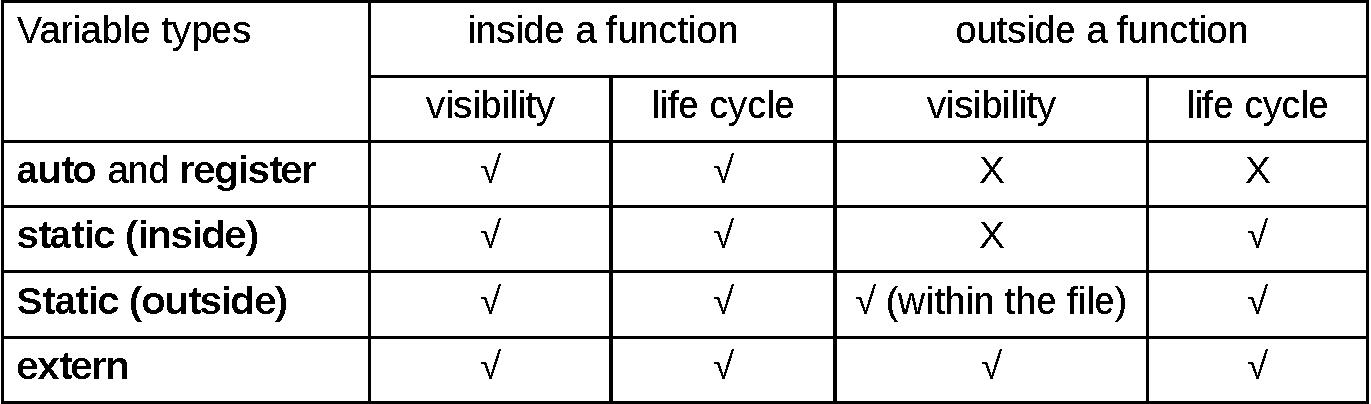
\includegraphics[width=0.8\linewidth]{figs/extern_var_eng.pdf}
\end{figure}
\begin{itemize}
	\item {It is NOT recommended to use global variables}
	\item {Advantage: you can transfer value easily}
	\item {Darkside}
	\begin{itemize}
		\item {You do NOT know where they have been changed}
		\item {Hard to debug your code}
		\item {Your code will be very messy!!!}
	\end{itemize}
\end{itemize}
\end{frame}
\section{Variable Input/Output}
\label{sec:io}
\begin{frame}<beamer>
    \frametitle{Outline}
    \tableofcontents[currentsection]
\end{frame}

\begin{frame}[fragile]{printf() with placeholders (1)}
	\begin{itemize}
		\item {\textbf{printf("\%d ...\%f ...\%ld", d1, d2, d3)}}
		\item {A function \textbf{pre-defined} by C}
		\item {It is in charge of print things onto screen}
		\item {You should organize your things in special format}
	\end{itemize}
\begin{columns}	
\begin{column}{0.6\linewidth}
    [\textbf{Codes}]
	\begin{lstlisting}[numbers=none, language=c]
#include <stdio.h>
int main()
{
   int a = 1;
   float b = 3.1;
   char c = 'h';
   printf("a: %d\n", a);
   printf("b: %f\n", b);
   printf("c: %c\n", c);
   printf("a: %d, c: %c\n", a, c);
}
\end{lstlisting}
\end{column}
\begin{column}{0.3\linewidth}
[\textbf{Output}]
\begin{lstlisting}[numbers=none, language=c]
a: 1
b: 3.1
c: h
a: 1, c: h
\end{lstlisting}
\end{column}
\end{columns}
\end{frame}

\begin{frame}[fragile]{printf() with placeholders (2)}
	\begin{itemize}
		\item {``\%x" is called placeholder}
		\item {It \textbf{holds/occupies} the place that is replaced by output data}
		\item {Different output data require different placeholders}
		\item {The \textbf{order} of placeholders corresponds to the order of output}
		\item {The \textbf{number} of placeholders corresponds to the number of output}
	\end{itemize}
\begin{columns}	
\begin{column}{0.77\linewidth}
    [\textbf{Codes}]
	\begin{lstlisting}[numbers=none, language=c]
#include <stdio.h>
int main()
{
  int a = 3;
  int b = 5;
  float c = 7.4;
  printf("a: %d\nb: %d\nc: %f\n", a, b, c);
}
	\end{lstlisting}
\end{column}
\begin{column}{0.15\linewidth}
[\textbf{Output}]
\begin{lstlisting}[numbers=none, language=c]
a: 3
b: 5
c: 7.4
\end{lstlisting}
\end{column}
\end{columns}
\end{frame}

\begin{frame}{Supported placeholders}
\begin{itemize}
	\item {The placeholder determines how the value is interpreted.}
\end{itemize}
	\begin{tabular}{|c|c|c|}
		\hline
		\textbf{type} & \textbf{description} & \textbf{type of argument} \\\hline
		\%c & single character & char, int (if $<=$ 255) \\\hline
		\%d & decimal number & char, int \\\hline
		\%u & unsigned decimal number & unsigned char, unsigned int \\\hline
		\%x & hexadecimal number & char, int \\\hline
		\%ld & long decimal number & long \\\hline
		\%f & floating point number & float, double \\\hline
		\%lf & double number & double \\\hline
	\end{tabular}
\end{frame}

\begin{frame}[fragile]{printf() by example}
	\begin{itemize}
		\item {\textbf{printf("\%d ...\%f ...\%ld", d1, d2, d3)}}
		\item {A function \textbf{pre-defined} by C}
	\end{itemize}
\begin{columns}	
\begin{column}{0.6\linewidth}
    [\textbf{Codes}]
	\begin{lstlisting}[numbers=none, language=c]
#include <stdio.h>
int main()
{
   int a = 79;
   char b = 'n';
   printf("a: %d, b: %d\n", a, b);
   printf("a: %c, b: %c\n", a, b);
   printf("a: %x, b: %x\n", a, b);
}
	\end{lstlisting}
\end{column}
\begin{column}{0.35\linewidth}
[\textbf{Output}]

\end{column}
\end{columns}
\end{frame}

\begin{frame}[fragile]{printf() by example}
	\begin{itemize}
		\item {\textbf{printf("\%d ...\%f ...\%ld", d1, d2, d3)}}
		\item {A function \textbf{pre-defined} by C}
	\end{itemize}
\begin{columns}	
\begin{column}{0.6\linewidth}
    [\textbf{Codes}]
	\begin{lstlisting}[numbers=none, language=c]
#include <stdio.h>
int main()
{
  int a = 79;
  char b = 'n';
  printf("a: %d, b: %d\n", a, b);
  printf("a: %c, b: %c\n", a, b);
  printf("a: %x, b: %x\n", a, b);
}
	\end{lstlisting}
\end{column}
\begin{column}{0.35\linewidth}
[\textbf{Output}]
\begin{lstlisting}[numbers=none, language=c]
a: 79, b: 110
a: O, b: n
a: 4f, b: 6e
\end{lstlisting}
\end{column}
\end{columns}
\end{frame}

\begin{frame}{Escape Character in ASCII (1)}
\begin{itemize}
	\item {There are some special character to be print out}
	\begin{itemize}
		\item {``Tab'', ``Enter'', ``backspace''}
	\end{itemize}
	\item {We want to express it by one character in ASCII}
	\begin{itemize}
		\item {But....}
		\item {All characters have their own use}
	\end{itemize}
	\item {If we want to use them to express different meaning}
	\begin{itemize}
		\item {We use `$\diagdown$'}
	\end{itemize}
\end{itemize}
\end{frame}


\begin{frame}{Escape Character in ASCII (2)}
\vspace{-0.1in}
\begin{itemize}
	\item {All characters have their own use}
	\item {If we want to use them to express different meaning}
	\begin{itemize}
		\item {We use `$\backslash$'}
	\end{itemize}
\end{itemize}
\vspace{-0.1in}
\begin{table}
\begin{center}
	\begin{tabular}{|c|l|} \hline
	ESC & their charactor  \\ \hline
	`$\backslash$t' & Tab \\ \hline
	`$\backslash$b' & back one character \\ \hline
	`$\backslash$r' & return to the start if a line\\ \hline
	`$\backslash$n' & go to the next line\\ \hline
	`$\backslash\backslash$' & $\backslash$\\ \hline
	`$\backslash$'' & single quote: '\\ \hline
	`$\backslash$"' & double quote: "\\ \hline
	\end{tabular}
\end{center}
\end{table}
\vspace{-0.1in}
\begin{itemize}
	\item {Remember that it is one character: $\backslash$"}
	\item {It is valid: '$\backslash$b'}
\end{itemize}

\end{frame}


\begin{frame}[fragile]{Variable input}
	\begin{itemize}
		\item {\textbf{scanf("\%d...\%f", \&a, \&b)} is another useful function}
		\item {Like \textbf{printf}(), it is declared in \textbf{stdio.h}}
		\item {Like \textbf{printf}(), it has a format string with placeholders}
		\item You can use it to read values of primitive datatypes from the command line
	\end{itemize}
	\ \\ \ \\ Example:
	\begin{lstlisting}[numbers=none, language=c, frame=none]
		int i;
		scanf("%d", &i);	
	\end{lstlisting}
	\begin{itemize}
		\item {Notice that there is ``\&'' before the variable}
		\item {This \textbf{operator} takes the address of the variable}
		\item {When buy goods online, you should put your the address}
		\item {The postman will transfer the \textbf{goods} (value) to your \textbf{mailbox} (variable)}
	\end{itemize}
\end{frame}

\begin{frame}{Notes for scanf}
	\begin{itemize}
		\item {\textbf{scanf}() uses the same placeholders as \textbf{printf}()}
		\item {You must type an \textcolor{red}{\textit{\&}} before each variable identifier}
		\item {If you read a number (using \%d, \%u etc.), interpretation}
		\begin{itemize}
			\item {Starts at first digit}
			\item {Ends before last \textbf{non digit} character}
			\item {E.g: \textbf{2} \textbf{2.3}}
		\end{itemize}
		\item {If you use \%c, the first character of the user input is taken}
	\end{itemize}
\end{frame}

\begin{frame}[fragile]{scanf() by example}
	\begin{itemize}
		\item {\textbf{scanf("\%d ...\%f ...\%ld", \&d1, \&d2, \&d3)}}
		\item {A function \textbf{pre-defined} by C}
	\end{itemize}
\begin{columns}	
\begin{column}{0.6\linewidth}
    [\textbf{Codes}]
	\begin{lstlisting}[numbers=none, language=c]
#include <stdio.h>
int main()
{
   int a = 79;
   float b = 0.1;
   printf("a: %d, b: %f\n", a, b);
   printf("Input a and b: ");
   scanf("%d%f", &a, &b);
   printf("a: %d, b: %f\n", a, b);
}
	\end{lstlisting}
\end{column}
\begin{column}{0.35\linewidth}
[\textbf{Output}]
	\begin{lstlisting}[numbers=none, language=c]
a: 79, b: 0.1
Input a and b: xx xx.xx
a: xx, b: xx.xx
	\end{lstlisting}
\end{column}
\end{columns}
\end{frame}
\section{Data Operators and Expressions}
\label{sec:oper}
\begin{frame}<beamer>
    \frametitle{Outline}
    \tableofcontents[currentsection]
\end{frame}

\begin{frame}[fragile]{Overview about Expressions}
\begin{itemize}
	\item {Legal expressions consist of legal combinations of}
	\begin{itemize}
		\item {Constants: const float PI = 3.14}
		\item {Variables: int a, b;}
		\item {Operators: +,-}
		\item {Function alls, printf("\%d", a)}
	\end{itemize}
\end{itemize}

\end{frame}

\begin{frame}[fragile]{Vadlid Operators in C}
\begin{itemize}
	\item {Operators}
	\begin{itemize}
		\item {Arithmetic: +,-,*, /, \%}
		\item {Relational: ==, !=, $>$,$<$, $<=$, $>=$}
		\item {Logical: \&\&, !, $||$}
		\item {\textcolor{yellow}{Bitwise}: \&, |, \^{ }, \~{ }}
		\item {\textcolor{yellow}{Shift}: $<<$, $>>$}
	\end{itemize}
\end{itemize}
\end{frame}

\begin{frame}[fragile]{Arithmetic Operators in C}
\begin{itemize}
	\item {Rules for operator precedence}
\end{itemize}
\begin{table}
\begin{center}
\begin{tabular}{|c|c|c|}
\hline 
Operator & Operation & Precedence \\ \hline \hline
() & Parenthese & Evaluated \textcolor{red}{first} \\ \hline
*,/ or \%&multiplication, division & evluated \textcolor{red}{second} \\ \hline
+ or - & addition, substraction & evaluated \textcolor{red}{last} \\ \hline
\hline
\end{tabular}
\end{center}
\end{table}
\begin{itemize}
	\item {Take average of three numbers}
	\item {1+2+4/3 ??}
\end{itemize}
\end{frame}

\begin{frame}[fragile]{Precedence Example}
\begin{equation}
(2+3+5)/3 \nonumber
\end{equation}
\begin{equation}
5*((2+6)%2) \nonumber
\end{equation}
\begin{columns}
\begin{column}{0.45\linewidth}
	\begin{lstlisting}[numbers=none, language=c]
	int avg = 2 + 3 + 5/3;
	float x=5*2+6%2;
	\end{lstlisting}
\end{column}
\begin{column}{0.45\linewidth}
	\begin{lstlisting}[numbers=none, language=c]
	int avg = (2 + 3 + 5)/3;
	float x=5*((2+6)%2);
	\end{lstlisting}
\end{column}
\end{columns}
\begin{itemize}
	\item {\textcolor{red}{Try to use ``()'' to clarify, if you are uncertain about the precedence}}
\end{itemize}
\end{frame}

\begin{frame}[fragile]{Division Operator (1)}
\begin{itemize}
	\item {Generates a result that is the same data type of \textcolor{red}{the largest operand} used in the operation}
	\item {Dividing two integers yields an integer result}
\end{itemize}
\begin{columns}
\begin{column}{0.4\linewidth}
	\begin{lstlisting}[numbers=none, language=c]
	5/2
	17/5
	\end{lstlisting}
\end{column}
\begin{column}{0.4\linewidth}
[Result]
	\begin{lstlisting}[numbers=none, language=c]
	2
	3
	\end{lstlisting}
\end{column}
\end{columns}
\end{frame}

\begin{frame}[fragile]{Division Operator (2)}
\begin{itemize}
	\item {Generates a result that is the same data type of \textcolor{red}{the largest operand} used in the operation}
	\item {Dividing two integers yields an integer result}
\end{itemize}
\begin{columns}
\begin{column}{0.4\linewidth}
	\begin{lstlisting}[numbers=none, language=c]
	5.0/2
	17.0/5
	\end{lstlisting}
\end{column}
\begin{column}{0.4\linewidth}
[Result]
	\begin{lstlisting}[numbers=none, language=c]
	2.5
	3.4
	\end{lstlisting}
\end{column}
\end{columns}
\end{frame}

\begin{frame}[fragile]{Modulus Operator \%}
\begin{itemize}
	\item {Modulus Operator \% returns the remainder}
	\item {Dividing two integers yields an integer result}
\end{itemize}
\begin{columns}
\begin{column}{0.4\linewidth}
	\begin{lstlisting}[numbers=none, language=c]
	5%2
	17%5
	12%3
	\end{lstlisting}
\end{column}
\begin{column}{0.4\linewidth}
[Result]
	\begin{lstlisting}[numbers=none, language=c]
	1
	2
	0
	\end{lstlisting}
\end{column}
\end{columns}
\end{frame}

\begin{frame}[fragile]{Evaluating Arithmetic Expressions (1)}
\begin{itemize}
	\item {See whether you can work out the answer}
\end{itemize}
\begin{columns}
\begin{column}{0.4\linewidth}
	\begin{lstlisting}[numbers=none, language=c]
	11/2
	11%2
	11/2.0
	5.0/2
	\end{lstlisting}
\end{column}
\begin{column}{0.4\linewidth}
[Result]
%	\begin{lstlisting}[numbers=none, language=c]
%
%	\end{lstlisting}
\end{column}
\end{columns}
\end{frame}


\begin{frame}[fragile]{Evaluating Arithmetic Expressions (2)}
\begin{itemize}
	\item {Check your answer}
\end{itemize}
\begin{columns}
\begin{column}{0.4\linewidth}
	\begin{lstlisting}[numbers=none, language=c]
	11/2
	11%2
	11/2.0
	5.0/2
	\end{lstlisting}
\end{column}
\begin{column}{0.4\linewidth}
[Result]
	\begin{lstlisting}[numbers=none, language=c]
	5
	1
	5.5
	2.5
	\end{lstlisting}
\end{column}
\end{columns}
\end{frame}

\begin{frame}[fragile]{Arithmetic Expressions (1)}
\begin{columns}
\begin{column}{0.4\linewidth}
[Arithmetic Expression]
\begin{equation}
	\begin{aligned}
	\frac{a}{b}\\
	2x \\
	\frac{x-7}{2+3y} \nonumber
	\end{aligned}
\end{equation}
\end{column}
\begin{column}{0.4\linewidth}
[Expression in C]
	\begin{lstlisting}[numbers=none, language=c]
	a/b
	2*x
	(x-7)/(2+3*y)
	\end{lstlisting}
\end{column}
\end{columns}
\end{frame}

\begin{frame}[fragile]{Arithmetic Expressions (2)}
\begin{columns}
\begin{column}{0.4\linewidth}
[Arithmetic Expression]
	\begin{lstlisting}[numbers=none, language=c, frame=none]
	2 * (-3)
	4 * 5 - 15
	4 + 2 * 5
	7/2
	7 / 2.0
	2 / 5
	2.0 / 5.0
	2 / 5 * 5
	2.0 + 1.0 + 5 / 2
	5 % 2
	4 * 5/2 + 5 % 2
	\end{lstlisting}
\end{column}
\begin{column}{0.4\linewidth}

\end{column}
\end{columns}
\end{frame}

\begin{frame}[fragile]{Arithmetic Expressions (3)}
\begin{columns}
\begin{column}{0.4\linewidth}
[Arithmetic Expression]
	\begin{lstlisting}[numbers=none, language=c, frame=none]
	2 * (-3)
	4 * 5 - 15
	4 + 2 * 5
	7/2
	7 / 2.0
	2 / 5
	2.0 / 5.0
	2 / 5 * 5
	2.0 + 1.0 + 5 / 2
	5 % 2
	4 * 5/2 + 5 % 2
	\end{lstlisting}
\end{column}
\begin{column}{0.4\linewidth}
[Results]
	\begin{lstlisting}[numbers=none, language=c, frame=none]
	-6
	5
	14
	3
	3.5
	0
	0.4
	0
	5.0
	1
	11
	\end{lstlisting}
\end{column}
\end{columns}
\end{frame}


\begin{frame}[fragile]{Data Assignment}
\begin{itemize}
	\item {Assig value to variable in accordance with its type}
\end{itemize}
\begin{columns}
\begin{column}{0.45\linewidth}
	\begin{lstlisting}[numbers=none, language=c, rulecolor=\color{blue}]
	int main()
	{ 
	   int a;
	   a = 2.99;
	   printf("a = %d", a);
	}
	\end{lstlisting}
\end{column}
\begin{column}{0.4\linewidth}
  [Output]
	\begin{lstlisting}[numbers=none, language=c, rulecolor=\color{blue}]
	a = 2
	\end{lstlisting}
\end{column}
\end{columns}
\begin{itemize}
	\item {Comments: above expression is valid, but \textcolor{red}{NOT} suggested}
\end{itemize}
\end{frame}

\begin{frame}[fragile]{Shortcut assignment Operators (1)}
\begin{table}
	\begin{center}
	\begin{tabular}{|l|l|} 
	\hline
	Assignment & Shortcut \\ \hline
	d = d - 4 & d-=4 \\ \hline
	e = e*5  & e *= 5 \\ \hline
	f = f/3 & f /= 3 \\ \hline
	g = g\%9 & g \%=9 \\ \hline \hline
	m = m*(5 + 3) & m *= 5+3 \\ \hline
	k = k/(5 + 1) & m /= 5+1 \\ \hline
	k = k/(5*7) & k /= 5*7 \\ \hline
	\end{tabular}
	\end{center}
\end{table}
\end{frame}

\begin{frame}[fragile]{Shortcut assignment Operators (2)}
\begin{columns}
\begin{column}{0.17\linewidth}
\end{column}
\begin{column}{0.65\linewidth}
	\begin{lstlisting}[numbers=none, language=c, rulecolor=\color{blue}]
		a += 4;		/* a = a + 4; */
		a -= 4;		/* a = a - 4; */
		a *= b;		/* a = a * b; */
		b /= 4+2;	/* b = b / (4+2); */
		b %= 2+3;	/* b = b % (2+3); */
	\end{lstlisting}
\end{column}
\begin{column}{0.17\linewidth}
\end{column}
\end{columns}
\end{frame}

\begin{frame}[fragile]{Shorthand Operators (1)}
\begin{itemize}
	\item {Incremental operator: \textbf{++}}
	\begin{itemize}
		\item {\textbf{i++} equivalent to \textbf{i = i+1}}
	\end{itemize}
	\item {Decremental operator: \textbf{--}}
	\begin{itemize}
		\item {\textbf{i--} equivalent to \textbf{i = i-1}}
	\end{itemize}
	\item {When they are used alone}
	\begin{itemize}
		\item {\textbf{i++} and \textbf{++i} behave the same as}
		\item {\textbf{i = i+1}}
		\item {Similar comment applies to \textbf{--}}
	\end{itemize}
\end{itemize}
\end{frame}

\begin{frame}[fragile]{Shorthand Operators (2)}
\begin{itemize}
	\item {When they appear in a compound expression, things are different}
	\item {\textbf{a=i++} will be different from \textbf{a=++i}}
	\item {In \textbf{a=i++}, \textbf{i} contributes its value to \textbf{a} first, then self-increments}
	\item {In \textbf{a=++i}, \textbf{i} self-increments first, then contributes its value to \textbf{a}}
	\item {Similiar comments apply to \textbf{i--} and \textbf{--i}}
\end{itemize}
\begin{columns}
\begin{column}{0.45\linewidth}
	\begin{lstlisting}[numbers=none, language=c, rulecolor=\color{blue}]
	int main()
	{
	   int a, b, i = 4;
	   a = i++;
	   b = ++i;
	}
	\end{lstlisting}
\end{column}
\begin{column}{0.45\linewidth}
	\begin{lstlisting}[numbers=none, language=c, rulecolor=\color{blue}]
	int main()
	{
	   int a, i = 4;
	   a = i;
	   i = i + 1;
	   i = i + 1;
	   b = i;
	}
	\end{lstlisting}
\end{column}
\end{columns}
\end{frame}

\begin{frame}[fragile]{Shorthand Operators (3)}
\begin{itemize}
	\item {Now verify how much you understand}
\end{itemize}
\begin{columns}
\begin{column}{0.65\linewidth}
	\begin{lstlisting}[numbers=none, language=c, rulecolor=\color{blue}]
	int main()
	{
	   int a, b, i = 4;
	   a = i--;
	   b = --i;
	   printf("a = %d, b = %d\n", a, b);
	}
	\end{lstlisting}
\end{column}
\begin{column}{0.3\linewidth}
[Output]
	\begin{lstlisting}[numbers=none, language=c, rulecolor=\color{blue}]
	a = ?, b = ?
	\end{lstlisting}
\end{column}
\end{columns}
\end{frame}

\begin{frame}[fragile]{Conditional Operator}
\begin{itemize}
	\item {Conditional Operator: logic\_exp1?exp2:exp3}
	\item {Three operands}
	\item {If logic\_exp1 is \textcolor{green}{none zero}, takes \textbf{exp2}}
	\item {If logic\_exp1 is \textcolor{green}{zero}, takes \textbf{exp3}}
\end{itemize}
\begin{columns}
\begin{column}{0.65\linewidth}
	\begin{lstlisting}[numbers=none, language=c, rulecolor=\color{blue}]
	int main()
	{
	   int a = 2, b = 3, i = 4;
	   a = b>i?b:i;
	   b = b==3?2:1;
	   printf("a = %d, b = %d\n", a, b);
	}
	\end{lstlisting}
\end{column}
\begin{column}{0.3\linewidth}
[Output]
	\begin{lstlisting}[numbers=none, language=c, rulecolor=\color{blue}]
	a = 4, b = 2
	\end{lstlisting}
\end{column}
\end{columns}
\end{frame}
\section{Implicit and Forceful Data Type Casting}
\begin{frame}<beamer>
    \frametitle{Outline}
    \tableofcontents[currentsection]
\end{frame}

\begin{frame}[fragile]{Implicit Data Type Casting}
\begin{itemize}
	\item {See whether you can work out the answer}
\end{itemize}
\begin{columns}
\begin{column}{0.6\linewidth}
	\begin{lstlisting}[numbers=none, language=c, frame=none]
	char c = 'x';
	double a = c + 5 + 1.3 + 1.73e4;
	\end{lstlisting}
\end{column}
\begin{column}{0.4\linewidth}
\begin{figure}
	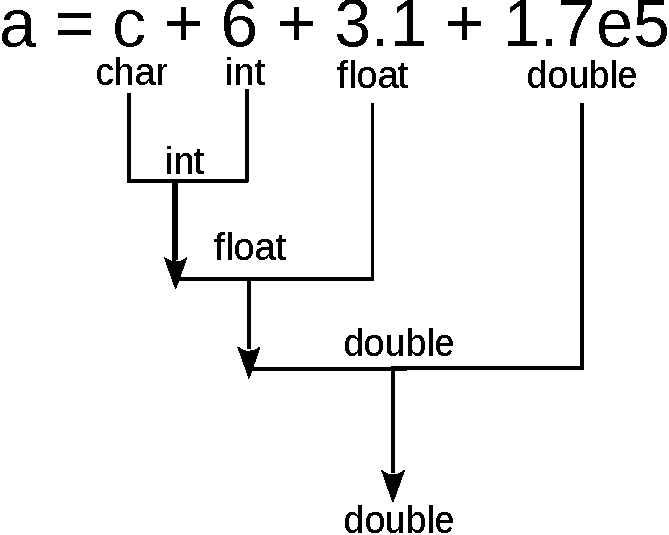
\includegraphics[width=0.9\linewidth]{figs/cast.pdf}
\end{figure}
\end{column}
\end{columns}
\begin{itemize}
	\item {Above type castings are done automatically (implicitly)}
	\item {Code below is risky, rear part will be truncated}
\end{itemize}
	\begin{lstlisting}[numbers=none, language=c, frame=none]
	int a = 0;
	a = 5.1;
	\end{lstlisting}
\end{frame}

\begin{frame}[fragile]{Explicit (forceful) Data Type Casting}
\begin{itemize}
	\item {See whether you can work out the answer}
\end{itemize}
\begin{columns}
\begin{column}{0.6\linewidth}
	\begin{lstlisting}[numbers=none, language=c, frame=none]
	char c = 'x';
	double a = (float)c + (float)5 + 1.3 + 1.73e4;
	\end{lstlisting}
\end{column}
\begin{column}{0.4\linewidth}
\begin{figure}
	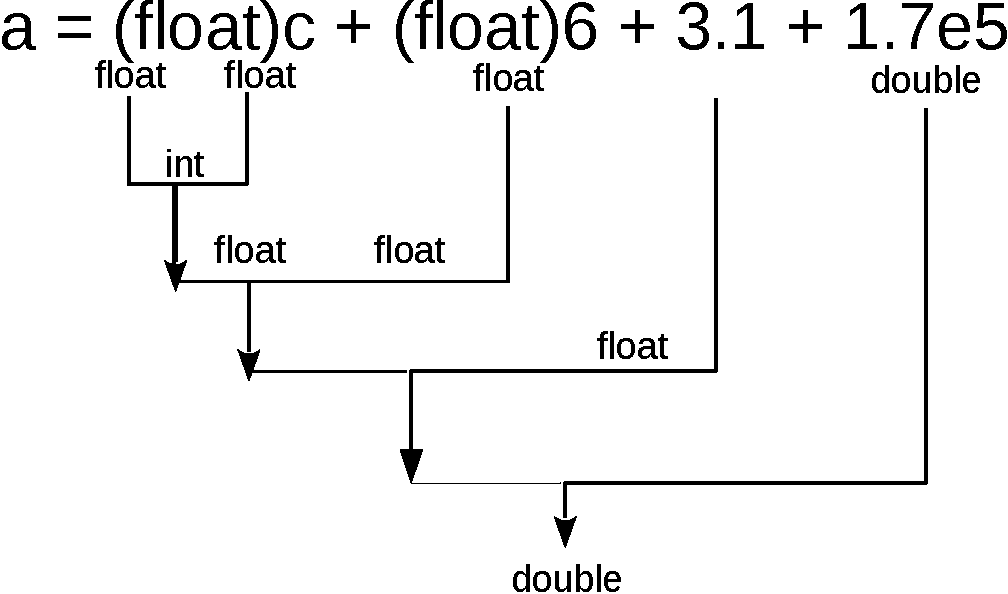
\includegraphics[width=0.9\linewidth]{figs/cast2.pdf}
\end{figure}
\end{column}
\end{columns}
\begin{itemize}
	\item {Above type castings are done forcefully}
	\item {Again it is risky sometimes}
\end{itemize}
\begin{columns}
\begin{column}{0.5\linewidth}
	\begin{lstlisting}[numbers=none, language=c, frame=none]
	int a = 0;
	float b = 5.4;
	a = (int)b;
	\end{lstlisting}
\end{column}
\begin{column}{0.5\linewidth}
	\begin{lstlisting}[numbers=none, language=c, frame=none]
	int a = 0;
	float b = 5.4;
	a = (int)round(b);
	\end{lstlisting}
\end{column}
\end{columns}
\end{frame}
\section{}
\end{document}
